%=============================================================================
%  POSTER — HỘI NGHỊ XÁC SUẤT & THỐNG KÊ
%  Ứng dụng phân tích thống kê đa biến trong dự báo rủi ro và đánh giá hiệu quả
%  thay huyết tương ở bệnh nhân viêm tụy cấp do tăng triglyceride
%
%  Biên dịch: pdfLaTeX (MiKTeX/TeX Live) — đúng như template của hội thảo.
%             XeLaTeX/LuaLaTeX cũng chạy được (nhánh fontspec bên dưới).
%  Hình:      thư mục figs_vn/ , sinh lại bằng:  python make_figures.py vn
%=============================================================================
% Luu y: trong baposter, fontscale LON hon = chu NHO hon (trang duoc dat o
% fontscale*khogiay roi phong to len). Template goc dung 0.30.
\documentclass[a0paper, portrait, final, fontscale=0.38]{baposter}

\usepackage{iftex}
\ifPDFTeX
  \usepackage[utf8]{inputenc}
  \usepackage[T5]{fontenc}
  \usepackage{palatino}
\else
  \usepackage{fontspec}
  \setmainfont{texgyrepagella}[Extension=.otf, UprightFont=*-regular,
    BoldFont=*-bold, ItalicFont=*-italic, BoldItalicFont=*-bolditalic]
\fi
\usepackage[vietnamese]{babel}

\usepackage{graphicx,calc}
\usepackage{amsmath,amssymb}
\usepackage{relsize}
\usepackage{multirow,multicol}
\usepackage{rotating,enumerate,floatflt}
\usepackage{bm,url,booktabs}

\newcommand{\captionfont}{\footnotesize}
\graphicspath{{figs_vn/}{images/}{../images/}}
\usetikzlibrary{calc}

\setlength{\columnsep}{1.0em}
\setlength{\columnseprule}{0mm}

\newcommand{\compresslist}{%
	\setlength{\itemsep}{1pt}%
	\setlength{\parskip}{0pt}%
	\setlength{\parsep}{0pt}%
}

% ---- Bảng màu: đã kiểm tra tương phản và độ phân biệt với mù màu ----------
\definecolor{boxblue}{RGB}{0, 71, 146}
\definecolor{cviolet}{RGB}{58, 45, 132}
\definecolor{cteal}{RGB}{13, 110, 84}
\definecolor{corange}{RGB}{176, 70, 25}
\definecolor{cmagenta}{RGB}{154, 44, 85}
\definecolor{cgreen}{RGB}{11, 92, 45}
\definecolor{cgrey}{RGB}{82, 81, 78}
\definecolor{lblue}{RGB}{233, 240, 251}
\definecolor{lviolet}{RGB}{239, 237, 250}
\definecolor{lteal}{RGB}{229, 246, 240}
\definecolor{lorange}{RGB}{253, 238, 230}
\definecolor{lmagenta}{RGB}{252, 236, 242}
\definecolor{lgreen}{RGB}{232, 245, 235}
\definecolor{alb}{RGB}{42, 120, 214}
\definecolor{ffp}{RGB}{235, 104, 52}
\definecolor{sigred}{RGB}{199, 42, 41}

% ---- Tiện ích --------------------------------------------------------------
\newcommand{\hl}[1]{\textcolor{cviolet}{\textbf{#1}}}
\newcommand{\key}[1]{\textbf{\textcolor{sigred}{#1}}}
\newcommand{\figcap}[1]{\par\vspace{0.1em}{\scriptsize\textcolor{cgrey}{#1}}\par}
% Cột "số liệu chính": nhãn + giá trị lớn
\newcommand{\bignum}[3]{\raggedright{\footnotesize\textcolor{cgrey}{#1}}\\[-0.1em]
  {\Large\textbf{\textcolor{#3}{#2}}}\par\vspace{0.35em}}

\begin{document}

	\begin{poster}%
	{
		grid=false,
		colspacing=0.7em,
		headerColorOne = boxblue,
		borderColor=boxblue,
		textborder=faded,
		headerborder=open,
		headerfont = \color{white}\bfseries\Large,
		headershape=roundedright,
		headershade=plain,
		background=none,
		bgColorOne=white,
		boxshade=plain,
		boxColorOne=white,
		headerheight=0.095\textheight
	}
	% Logo trái
	{
\includegraphics[height = 9.6em]{Logo Đơn.png}}
	% Tiêu đề
	{\vspace{0.15em}
	 \LARGE \textbf{Ứng dụng phân tích thống kê đa biến trong dự báo rủi ro và đánh giá hiệu quả}\\[0.25em]
	 \LARGE \textbf{thay huyết tương ở bệnh nhân viêm tụy cấp do tăng triglyceride}\vspace{0.25em}}
	% Tác giả
	{ \Large Phan Thái Sơn$^{1}$, \ Phạm Hiếu Đan$^{2}$, \ Nguyễn Minh Toàn$^{3}$, \
	  Lưu Phúc Lợi$^{2}$, \ Hoàng Văn Quang$^{2,*}$ \\[0.15em]
	  \normalsize $^{1}$Bệnh viện Đại học Y Dược TP.\ Hồ Chí Minh \quad
	  $^{2}$Bệnh viện Thống Nhất \quad
	  $^{3}$Trường Dược, Đại học Y Dược TP.\ Hồ Chí Minh
	  \ \ ($^{*}$tác giả liên hệ)}
	% Logo phải
	{
\includegraphics[height = 9.6em]{LOGO KHOA - ĐỨNG - KHÔNG NỀN.png}}

	%=========================================================================
	% HÀNG 1 — BÀI TOÁN  |  PHƯƠNG PHÁP
	%=========================================================================
	\headerbox{\ \ Bài toán thống kê và mục tiêu}{name=problem,column=0,row=0,
		headerColorOne=boxblue,borderColor=boxblue}{
		{\small
		Thay huyết tương (TPE) được dùng để hạ nhanh triglyceride (TG) trong viêm tụy cấp
		do tăng triglyceride. Câu hỏi lâm sàng được đưa về \hl{ba bài toán thống kê}:
		\begin{itemize}\compresslist
			\item[\textcolor{boxblue}{\textbf{1.}}] \textbf{Dự báo rủi ro} --- hồi quy logistic
			      đa biến cho khả năng diễn tiến nặng.
			\item[\textcolor{boxblue}{\textbf{2.}}] \textbf{Đo hiệu quả} --- phân tích
			      \emph{bắt cặp} trước--sau trên cùng bệnh nhân.
			\item[\textcolor{boxblue}{\textbf{3.}}] \textbf{So sánh hai dịch thay thế} khi
			      \emph{không phân nhóm ngẫu nhiên} --- hiệu chỉnh gây nhiễu.
		\end{itemize}
		\vspace{0.2em}

		\textbf{Ba thách thức của bộ dữ liệu.}
		\key{(i)} $n=93$ với chỉ 15 biến cố, tức \textbf{2,5} biến cố trên mỗi biến số
		so với ngưỡng khuyến cáo 10; \ \key{(ii)} \textbf{33 kiểm định} chạy song song;
		\ \key{(iii)} dịch thay thế không được chỉ định ngẫu nhiên.
		\vspace{0.25em}

		\textbf{Mục tiêu.} Minh hoạ quy trình phân tích đa biến có \hl{kiểm soát sai số loại I}
		và \hl{kiểm tra độ vững}.}
	}

	\headerbox{\ \ Dữ liệu và quy trình phân tích thống kê}{name=method,column=1,span=2,row=0,
		headerColorOne=cviolet,borderColor=cviolet}{

		\begin{minipage}[t]{0.470\linewidth}\vspace{0pt}
		{\small
		\textbf{Dữ liệu.} 93 bệnh nhân, 359 biến số; hồi cứu, đa trung tâm.
		Albumin 5\%: \textcolor{alb}{\textbf{59 ca}} \ $\cdot$ \ FFP: \textcolor{ffp}{\textbf{34 ca}}.
		Nặng 15 ca, trung bình--nặng 78 ca.\\[0.3em]
		\textbf{Trình bày.} TB\,$\pm$\,ĐLC, thêm trung vị (Q1--Q3) khi không chuẩn;
		biến định tính $n$ (\%); mọi KTC là 95\%.\\[0.3em]
		\textbf{Nhóm so sánh.} Theo dịch ở lần TPE đầu tiên; 3 ca đổi dịch ở lần 2 được
		phân tích riêng khi kiểm tra độ vững.\\[0.3em]
		\textbf{Kết cục.} Độ nặng (nhị giá) cho bài toán dự báo; tỉ lệ giảm TG và ba thang
		điểm APACHE II, SOFA, BISAP cho bài toán hiệu quả.\\[0.3em]
		\textbf{Phần mềm.} Python (NumPy, SciPy). Toàn bộ số liệu và hình trên poster
		\hl{tái lập được} bằng một script duy nhất chạy trên dữ liệu gốc.}
		\end{minipage}%
		\hfill
		\begin{minipage}[t]{0.510\linewidth}\vspace{0pt}
		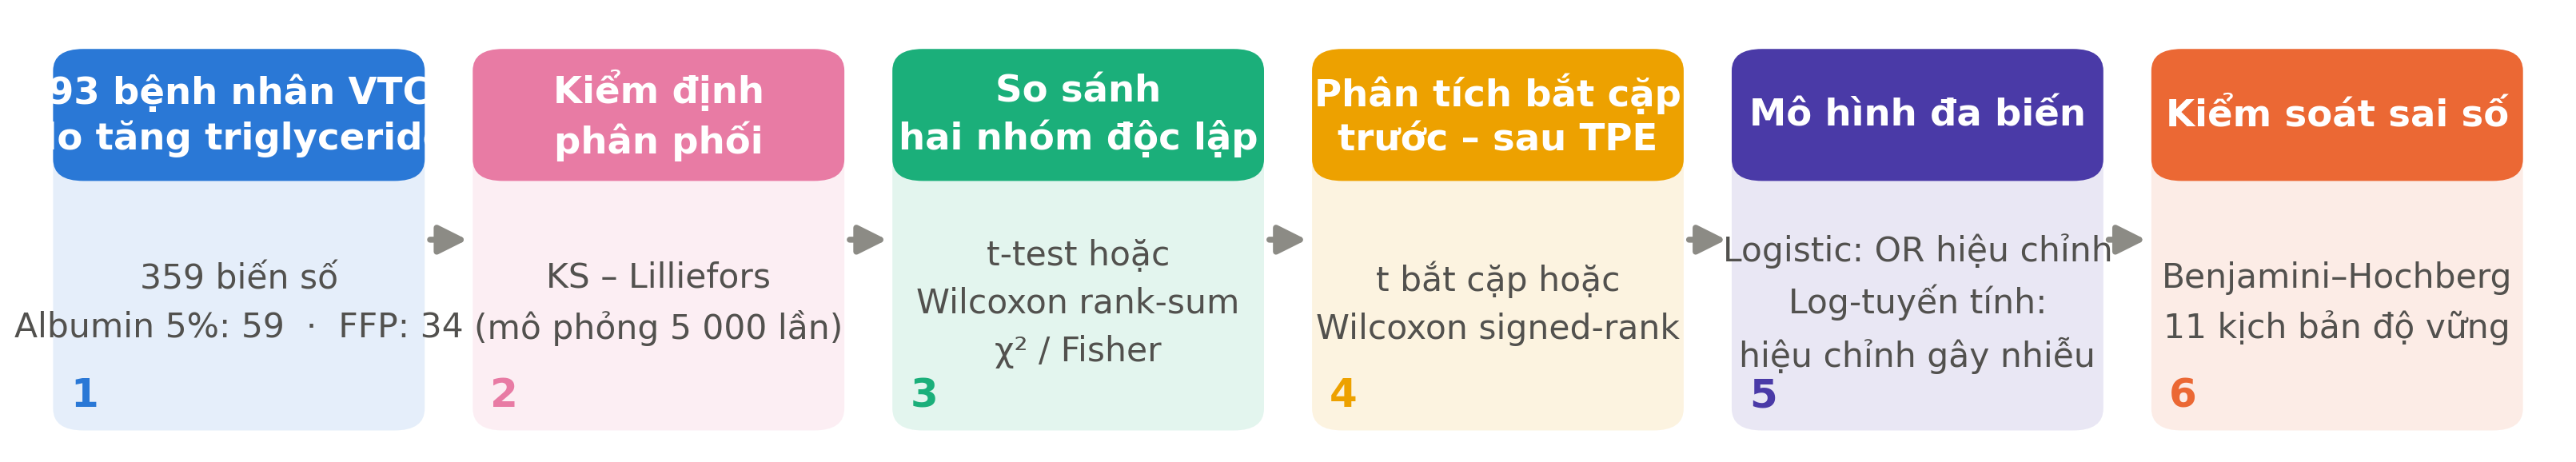
\includegraphics[width=\linewidth]{f0_pipeline.png}
		\figcap{\textbf{Quy trình 6 bước.} Phép kiểm chọn theo kết quả kiểm định phân phối ở bước 2;
		hai bước cuối dành cho kiểm soát sai số loại I và kiểm tra độ vững.}
		\end{minipage}
	}

	%=========================================================================
	% HÀNG 2 — KẾT QUẢ 1
	%=========================================================================
	\headerbox{\ \ Kết quả 1 --- Phân phối quyết định phép kiểm \ $\cdot$ \ Phân tích đơn biến độ nặng}%
		{name=kq1,column=0,span=3,row=0,below=problem,
		 headerColorOne=cteal,borderColor=cteal}{

		\begin{minipage}[t]{0.387\linewidth}\vspace{0pt}
		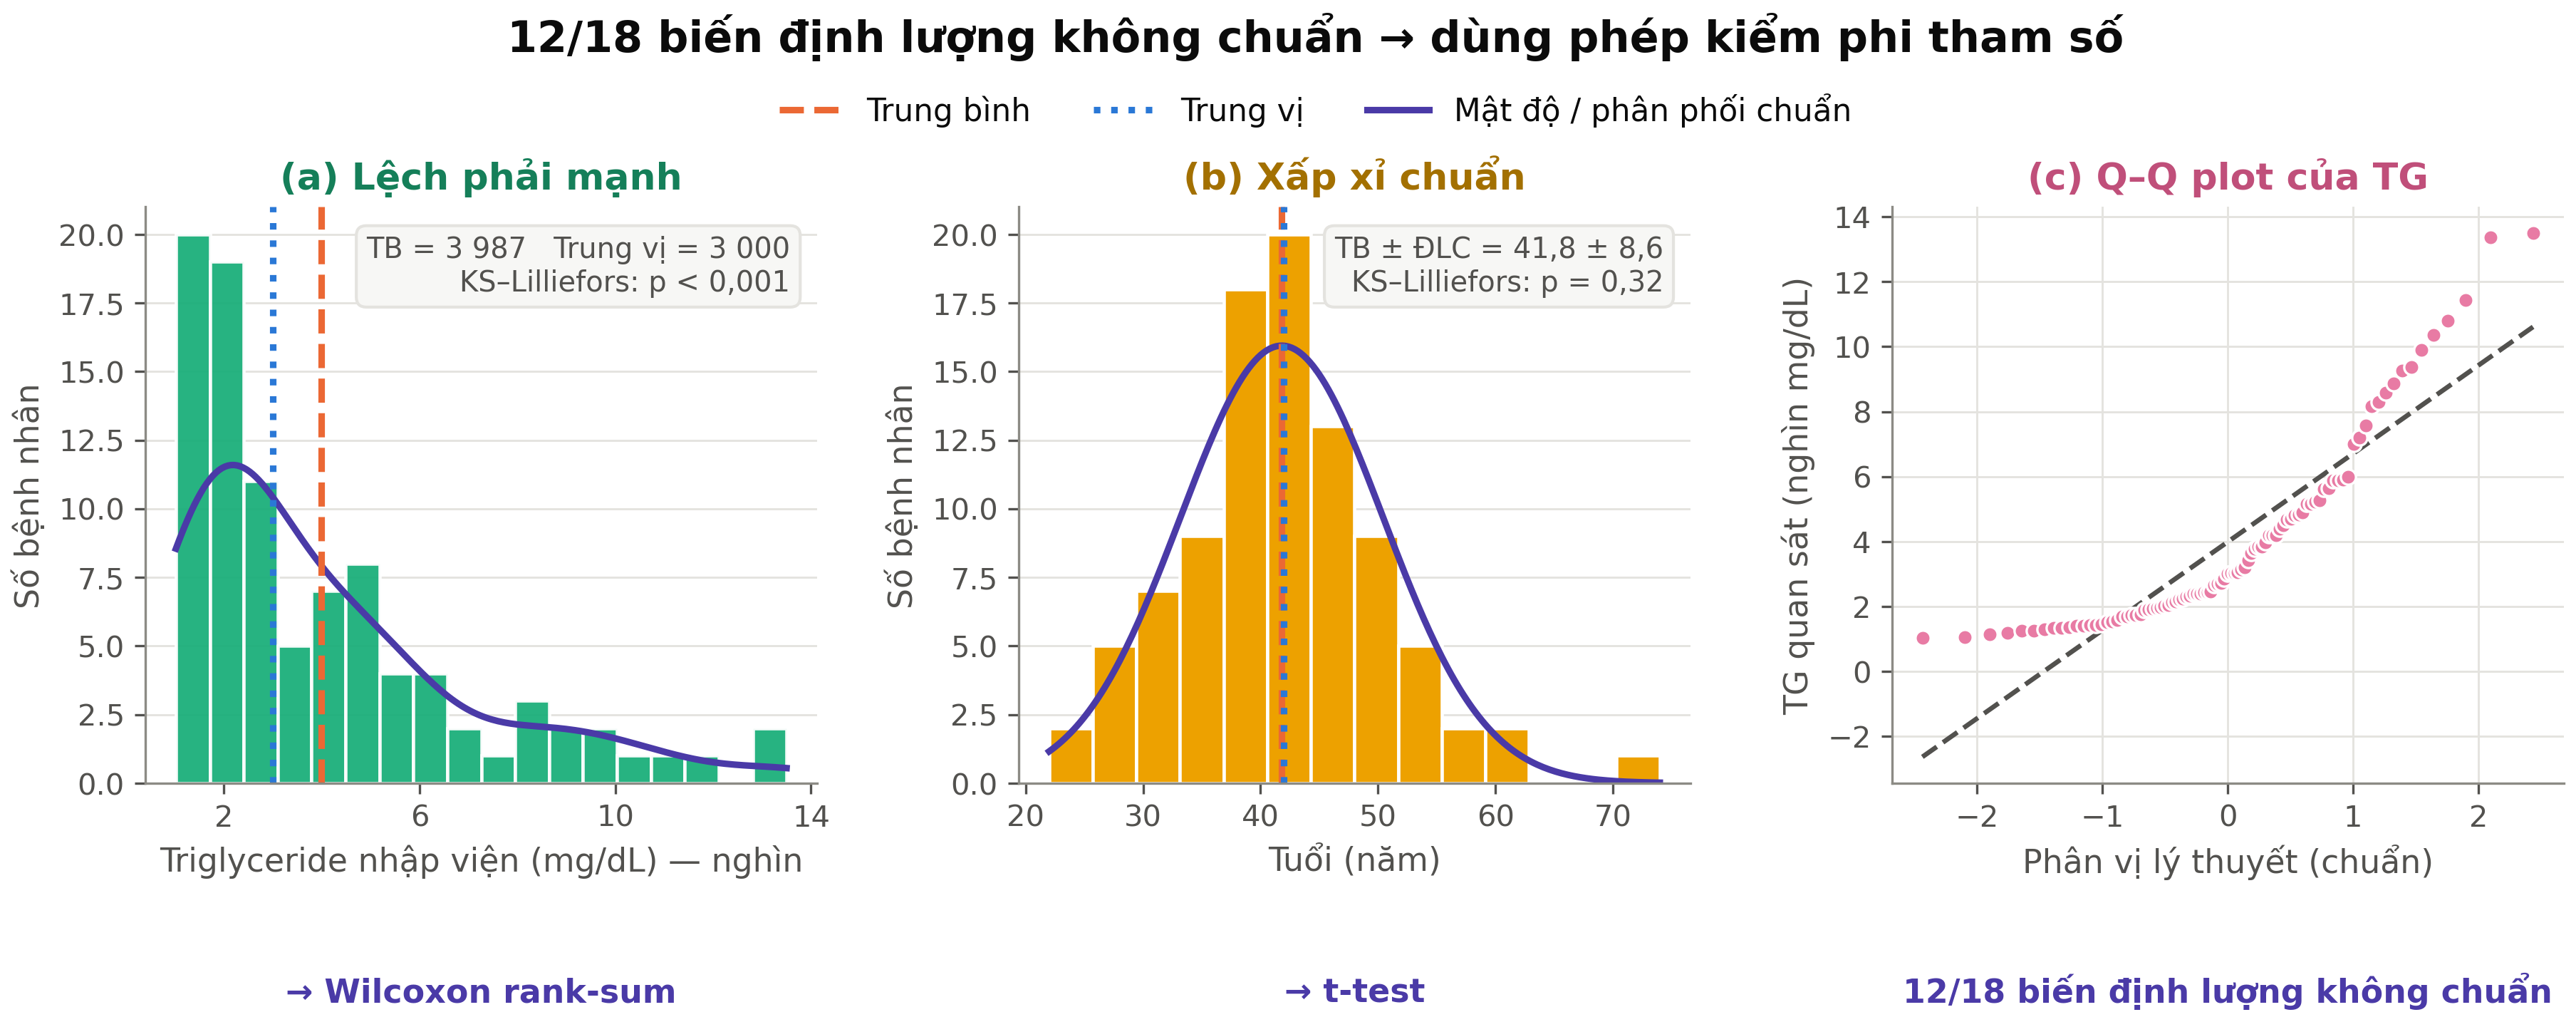
\includegraphics[width=\linewidth]{f1_distribution.png}
		\figcap{\textbf{Hình 1.} Kolmogorov--Smirnov hiệu chỉnh Lilliefors, p mô phỏng 5\,000 lần.
		\textbf{12/18} biến định lượng lệch chuẩn $\Rightarrow$ phi tham số là lựa chọn mặc định.}
		\end{minipage}%
		\hfill
		\begin{minipage}[t]{0.329\linewidth}\vspace{0pt}
		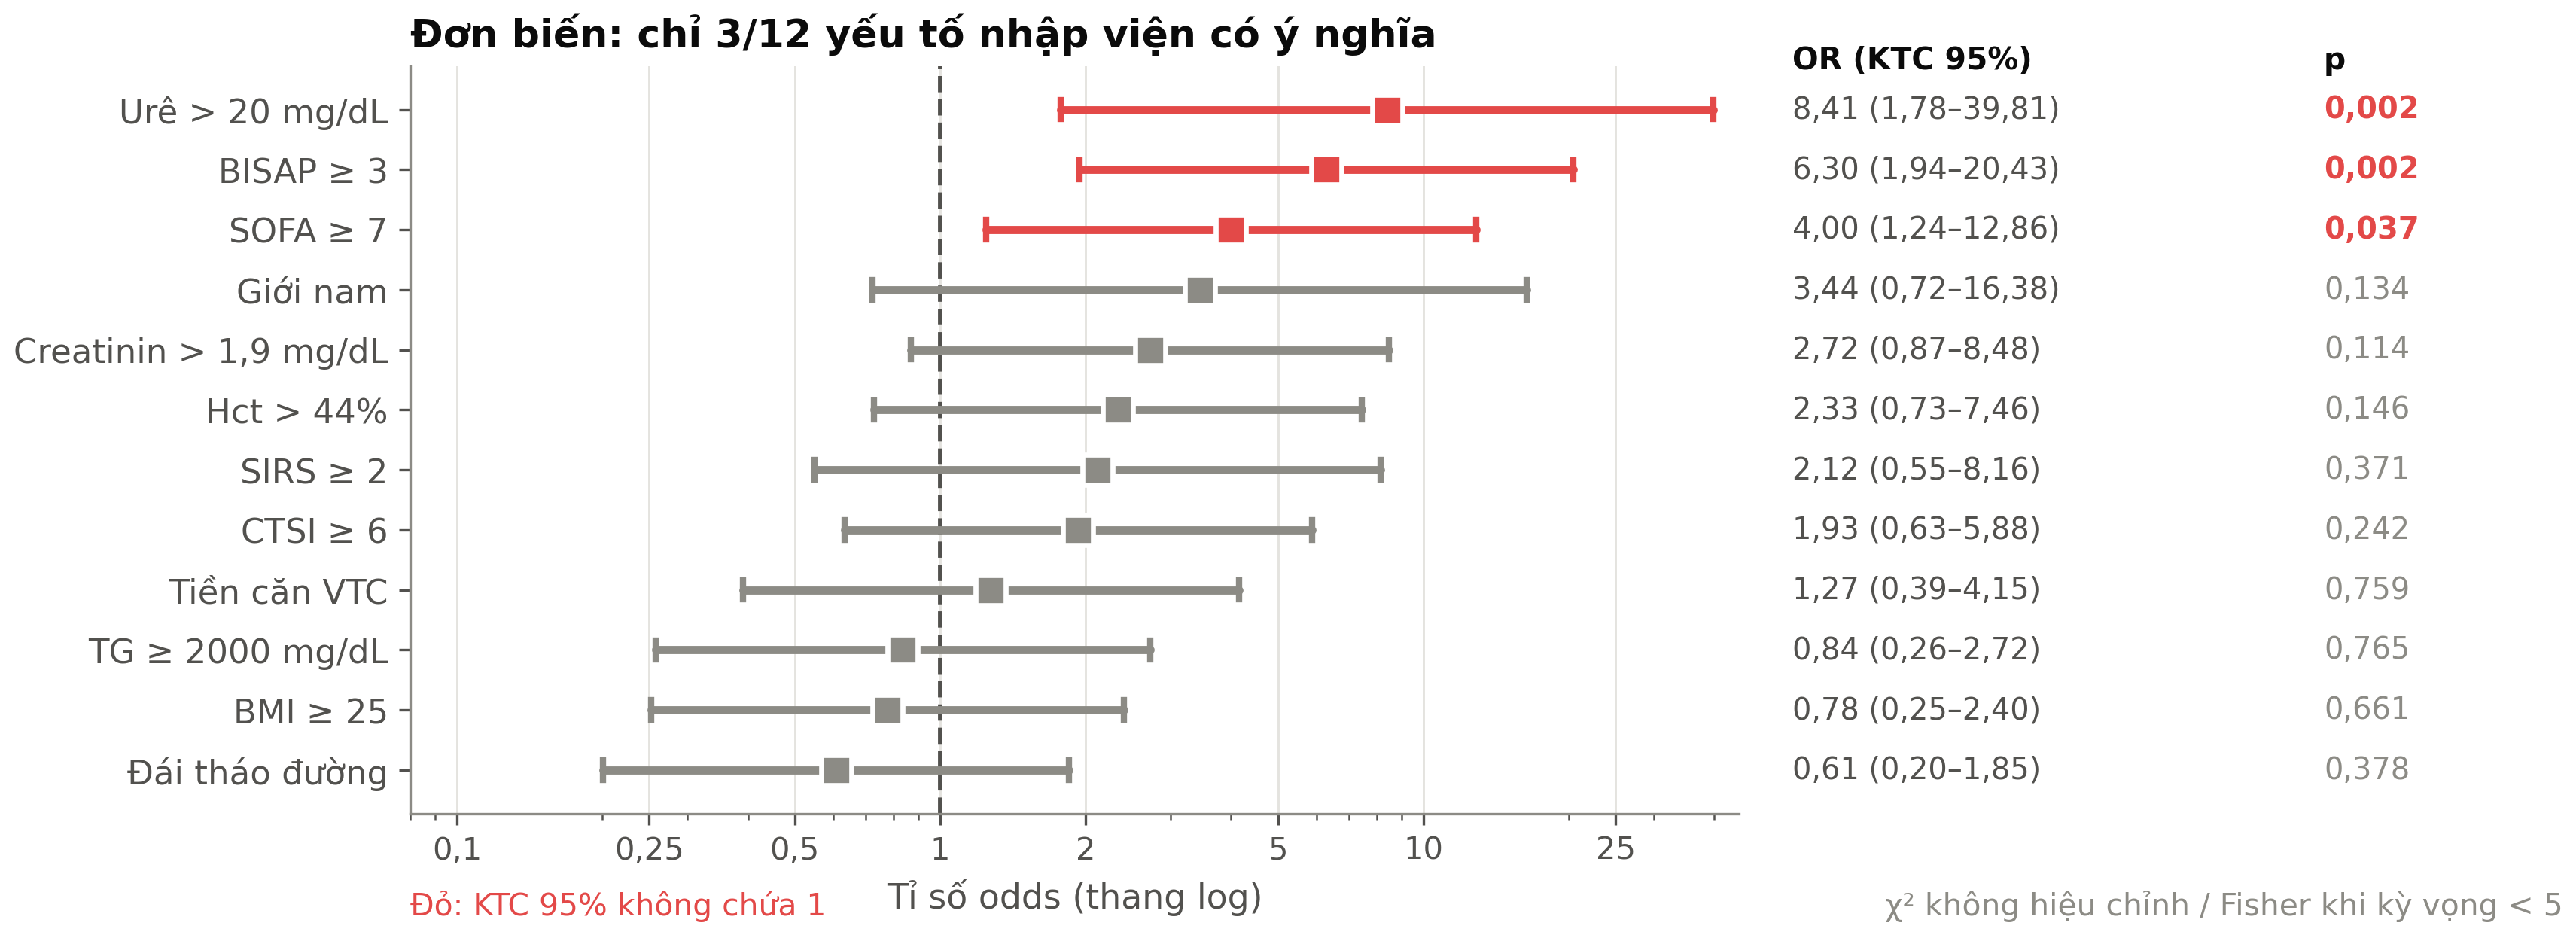
\includegraphics[width=\linewidth]{f3_forest_univariate.png}
		\figcap{\textbf{Hình 2.} OR thô của 12 yếu tố lúc nhập viện. Ba yếu tố có KTC 95\% không
		chứa 1; mọi KTC đều rất rộng --- hệ quả của 15 biến cố.}
		\end{minipage}%
		\hfill
		\begin{minipage}[t]{0.255\linewidth}\vspace{0pt}
		\colorbox{lteal}{\begin{minipage}{0.92\linewidth}\raggedright\vspace{0.3em}
		\bignum{Biến lệch chuẩn}{12 / 18}{cteal}
		\bignum{OR của BISAP $\geq3$}{6,30}{cteal}
		\bignum{KTC 95\%}{1,94 -- 20,43}{cgrey}
		\bignum{OR của SOFA $\geq7$}{4,00}{cteal}
		{\scriptsize\textcolor{cgrey}{Urê $>20$ mg/dL: OR 8,41 (1,78--39,81)}}
		\vspace{0.3em}\end{minipage}}
		\end{minipage}

		\vspace{0.15em}
		{\small \textcolor{cteal}{$\blacktriangleright$} \ \key{Cảnh báo diễn giải:}
		biến kết cục độ nặng được tính từ nhịp tim, nhịp thở và urê, trong khi BISAP và SIRS
		cũng dùng chính các thành phần này $\Rightarrow$ liên quan quan sát được
		\textbf{một phần do trùng định nghĩa}, không nên hiểu là khả năng tiên lượng độc lập.}
	}

	%=========================================================================
	% HÀNG 3 — KẾT QUẢ 2
	%=========================================================================
	\headerbox{\ \ Kết quả 2 --- Hồi quy logistic đa biến \ $\cdot$ \ Hiệu quả thay huyết tương (bắt cặp)}%
		{name=kq2,column=0,span=3,row=0,below=kq1,
		 headerColorOne=corange,borderColor=corange}{

		\begin{minipage}[t]{0.307\linewidth}\vspace{0pt}
		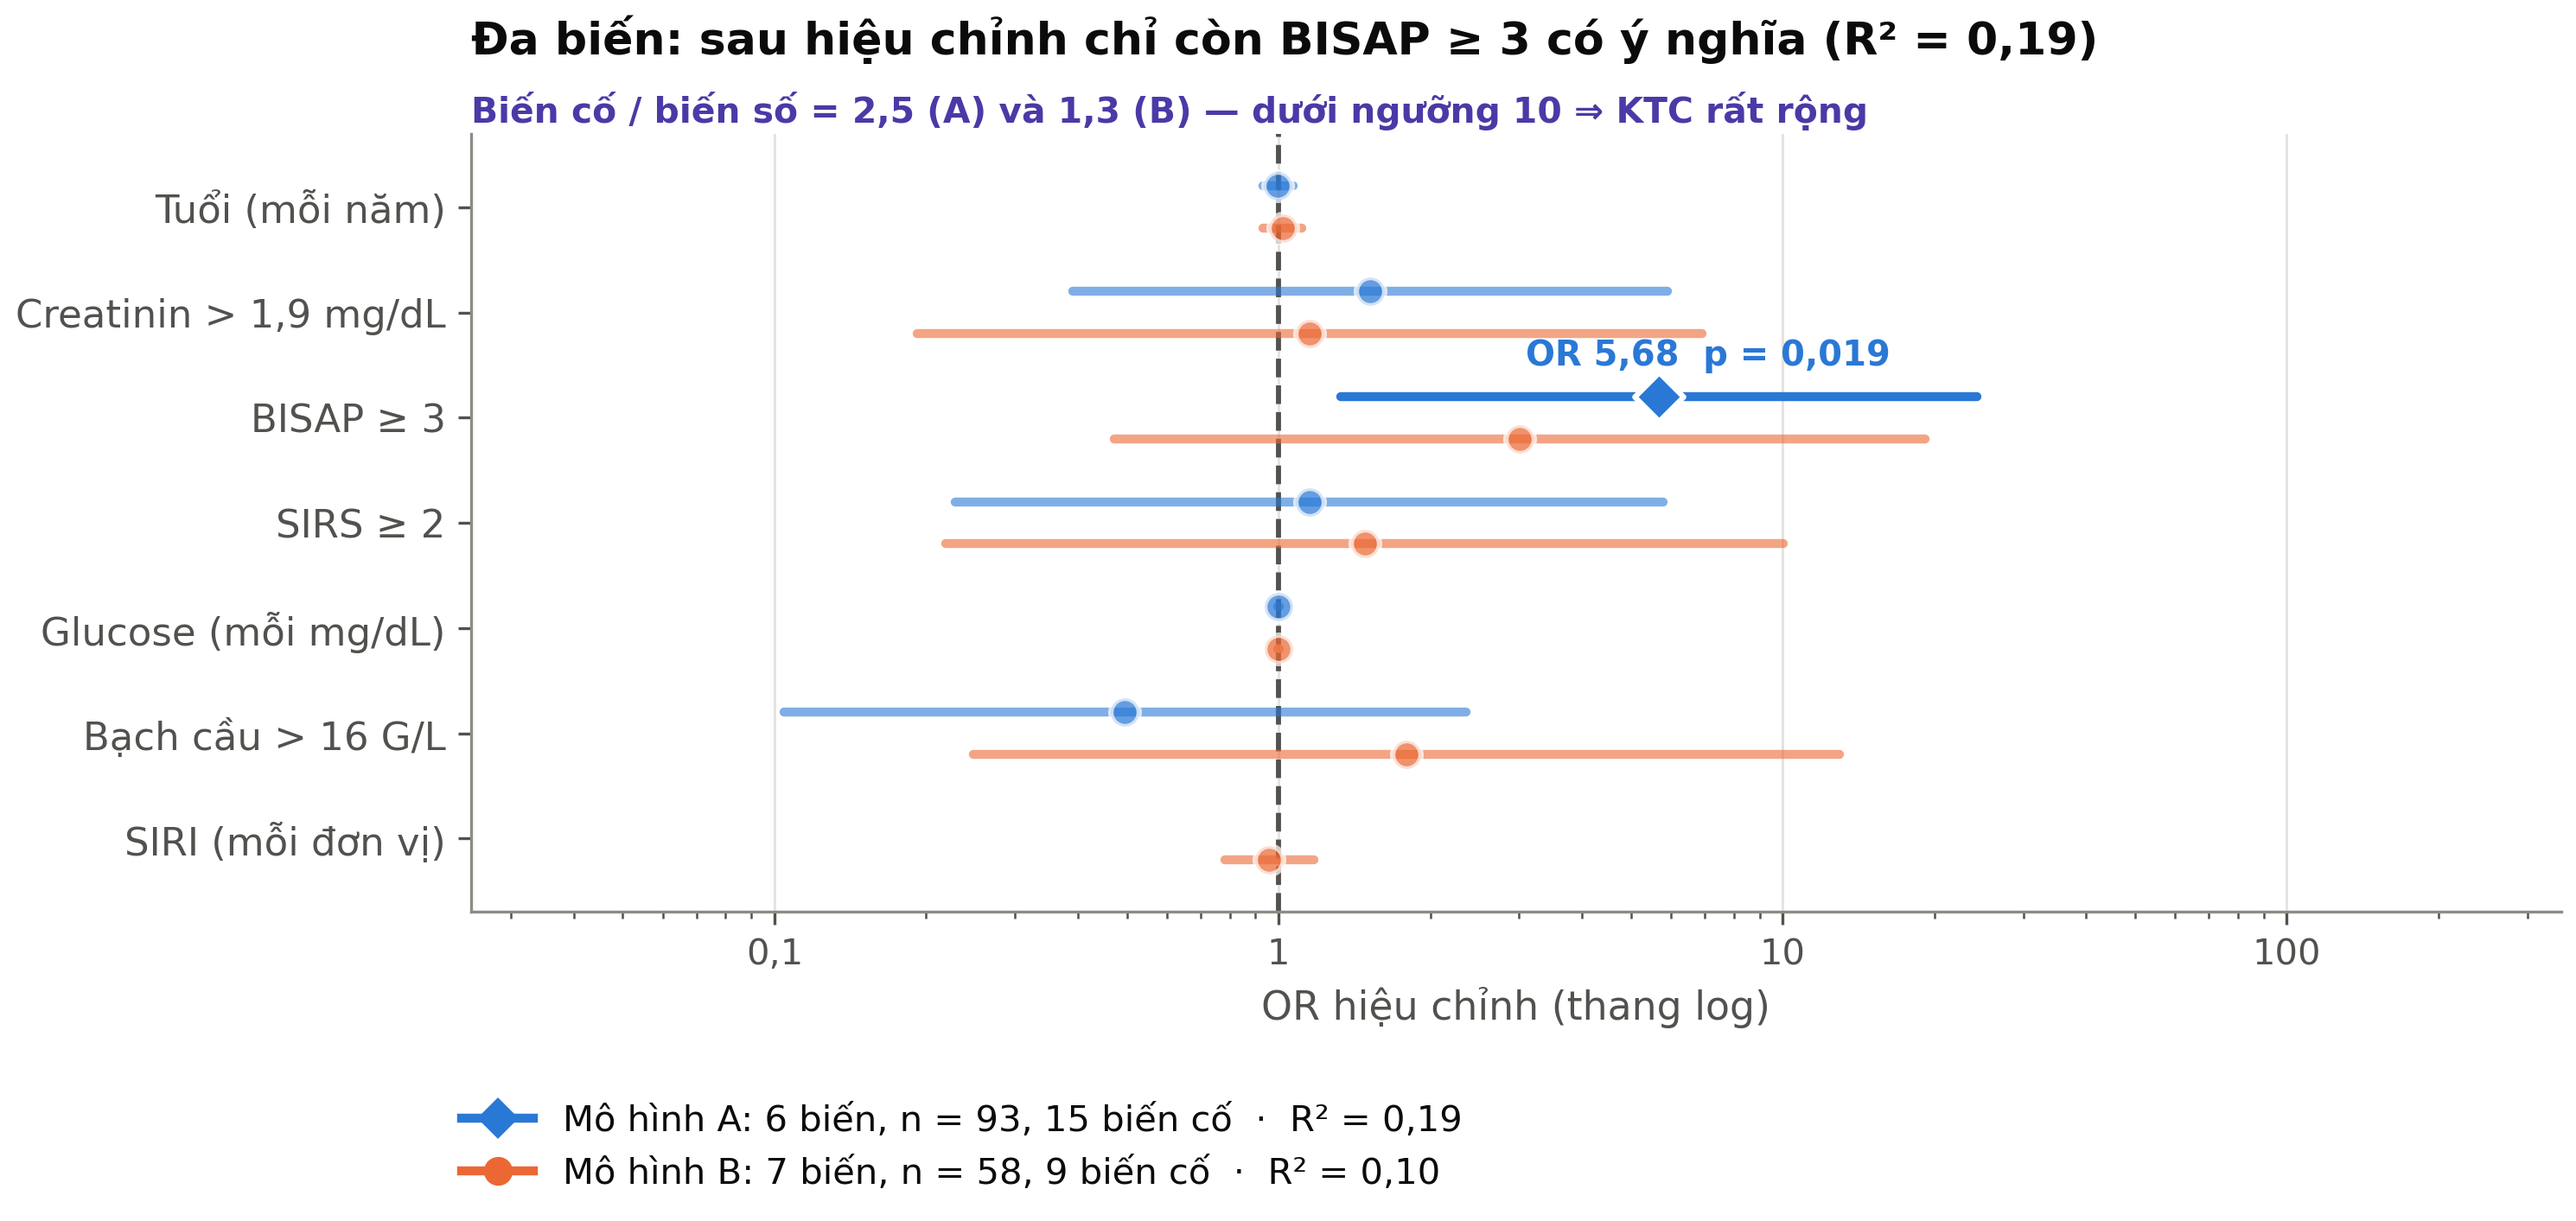
\includegraphics[width=\linewidth]{f4_forest_multivariable.png}
		\figcap{\textbf{Hình 3.} \textbf{Mô hình A} ($n=93$; 15 biến cố): chỉ BISAP $\geq3$ giữ ý
		nghĩa (OR 5,68; $R^{2}=0{,}19$). \textbf{Mô hình B} thêm SIRI: không biến nào có ý nghĩa.}
		\end{minipage}%
		\hfill
		\begin{minipage}[t]{0.435\linewidth}\vspace{0pt}
		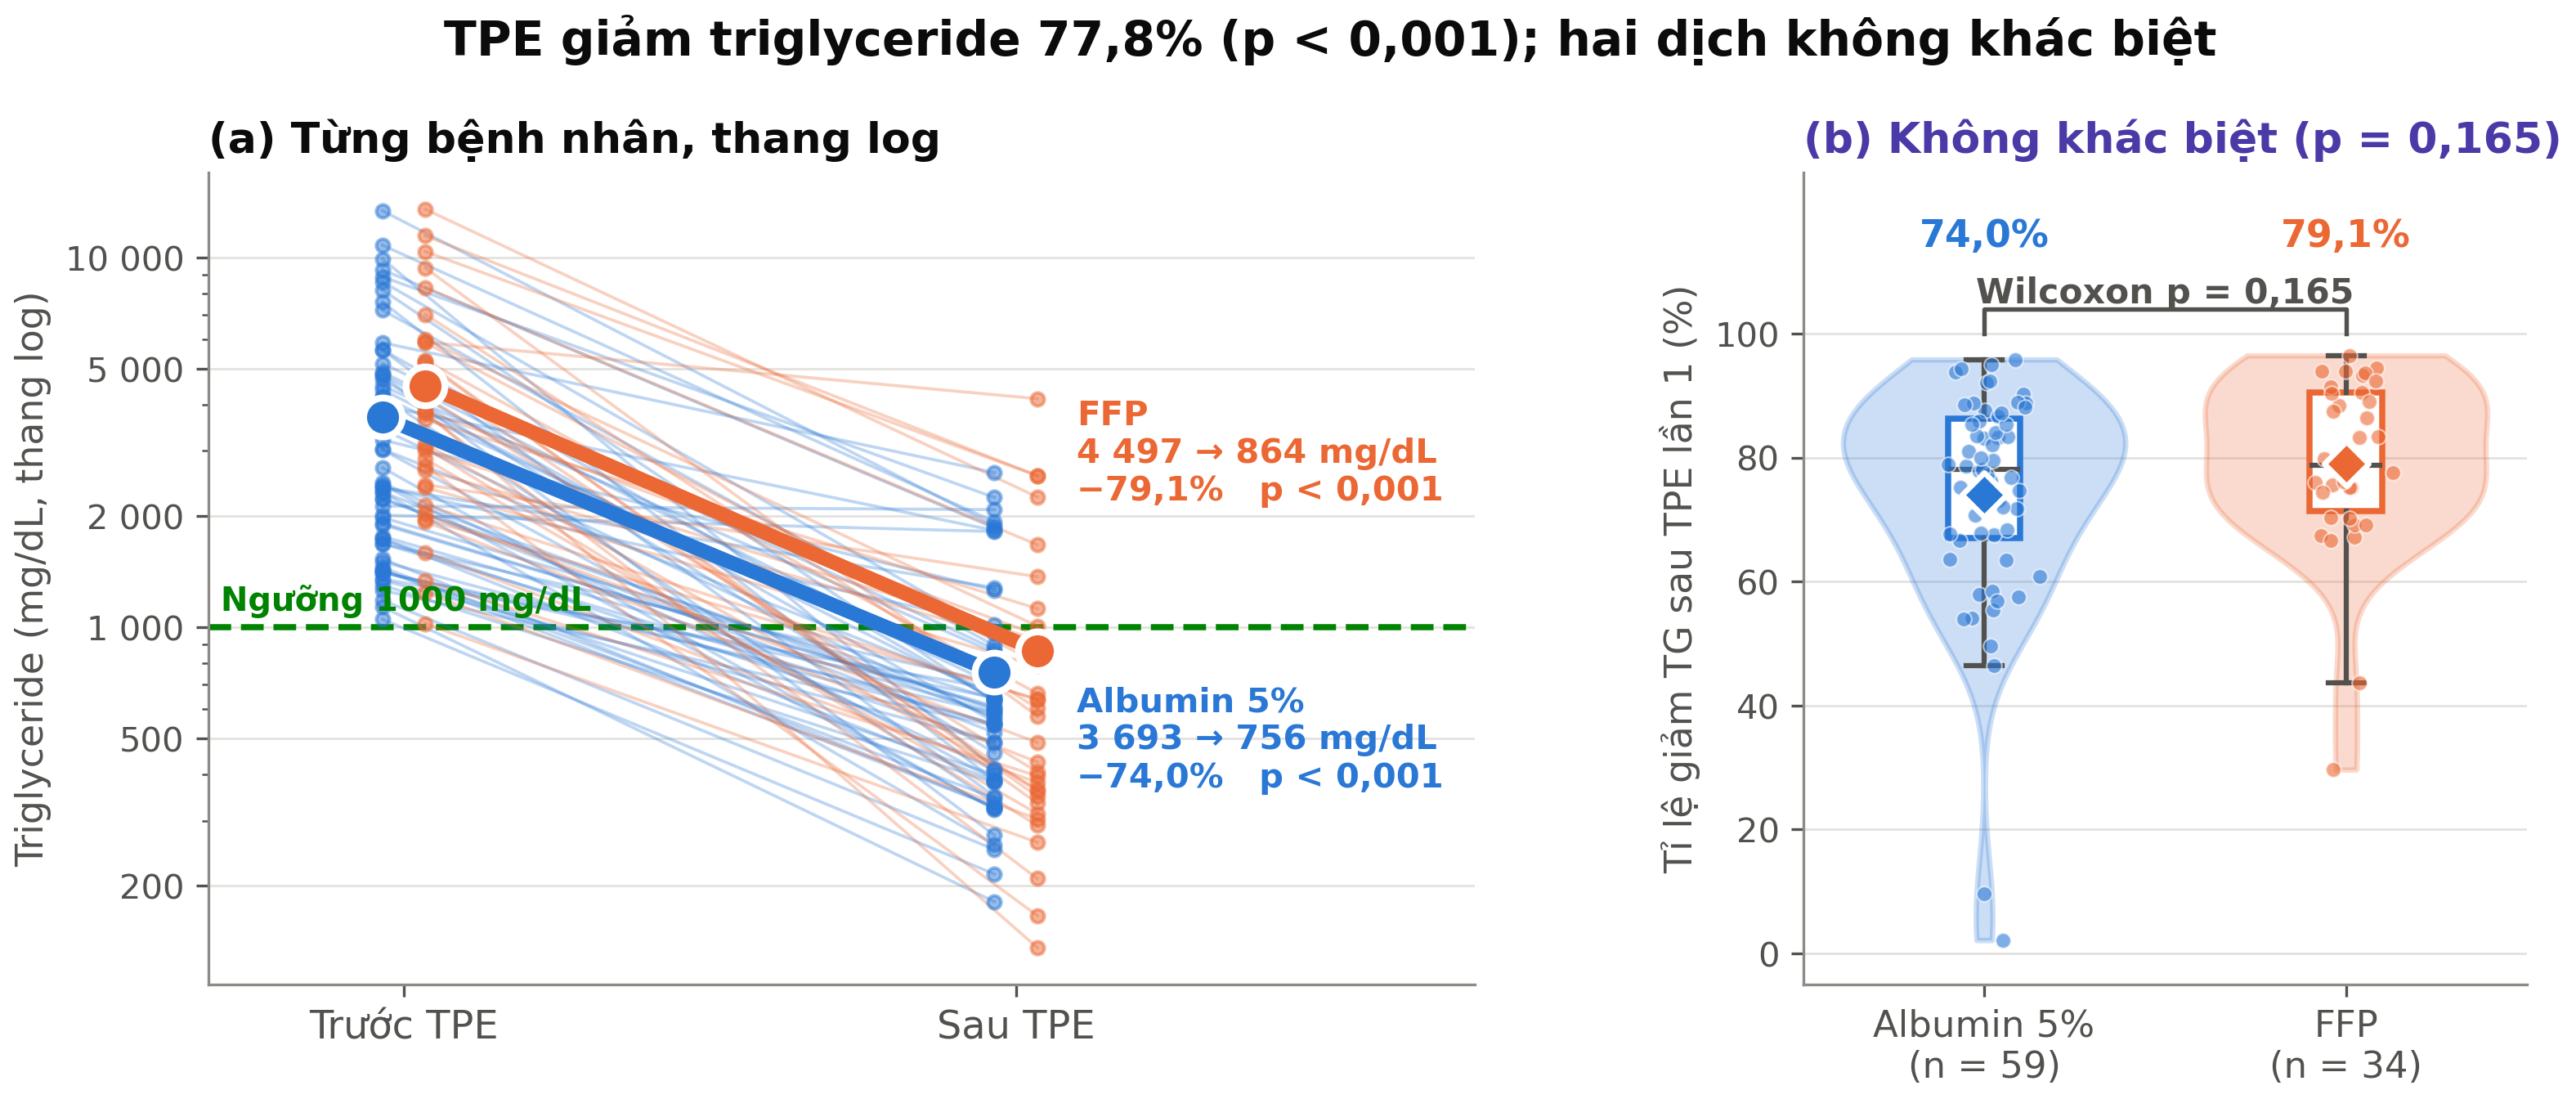
\includegraphics[width=\linewidth]{f5_paired_tg.png}
		\figcap{\textbf{Hình 4.} Wilcoxon signed-rank trên cùng bệnh nhân: $3\,987 \rightarrow 795$
		mg/dL ($-77{,}8\%$; $p<0{,}001$); \textbf{79,6\%} số ca đạt TG $<1000$ mg/dL sau lần 1.}
		\end{minipage}%
		\hfill
		\begin{minipage}[t]{0.255\linewidth}\vspace{0pt}
		\colorbox{lorange}{\begin{minipage}{0.92\linewidth}\raggedright\vspace{0.3em}
		\bignum{Giảm TG chung}{77,8\%}{corange}
		\bignum{APACHE II}{16,9 $\rightarrow$ 10,5}{corange}
		\bignum{SOFA}{4,2 $\rightarrow$ 3,4}{corange}
		\bignum{BISAP}{1,8 $\rightarrow$ 1,1}{corange}
		{\scriptsize\textcolor{cgrey}{Cả ba thang điểm: $p<0{,}001$, Wilcoxon bắt cặp, $n=93$}}
		\vspace{0.3em}\end{minipage}}
		\end{minipage}

		\vspace{0.15em}
		{\small \textcolor{corange}{$\blacktriangleright$} \ \key{Giới hạn của mô hình đa biến:}
		15 biến cố cho 6 biến số $\Rightarrow$ số biến cố trên mỗi biến chỉ \textbf{2,5}, thấp hơn
		nhiều ngưỡng 10 của Peduzzi. Ước lượng vì vậy không ổn định và KTC rất rộng: kết quả
		mang tính \textbf{thăm dò}, chưa đủ để xây dựng thang điểm tiên lượng.}
	}

	%=========================================================================
	% HÀNG 4 — KẾT QUẢ 3
	%=========================================================================
	\headerbox{\ \ Kết quả 3 --- Albumin 5\% so với FFP: hiệu chỉnh gây nhiễu \ $\cdot$ \ kiểm soát đa so sánh}%
		{name=kq3,column=0,span=3,row=0,below=kq2,
		 headerColorOne=cmagenta,borderColor=cmagenta}{

		\begin{minipage}[t]{0.339\linewidth}\vspace{0pt}
		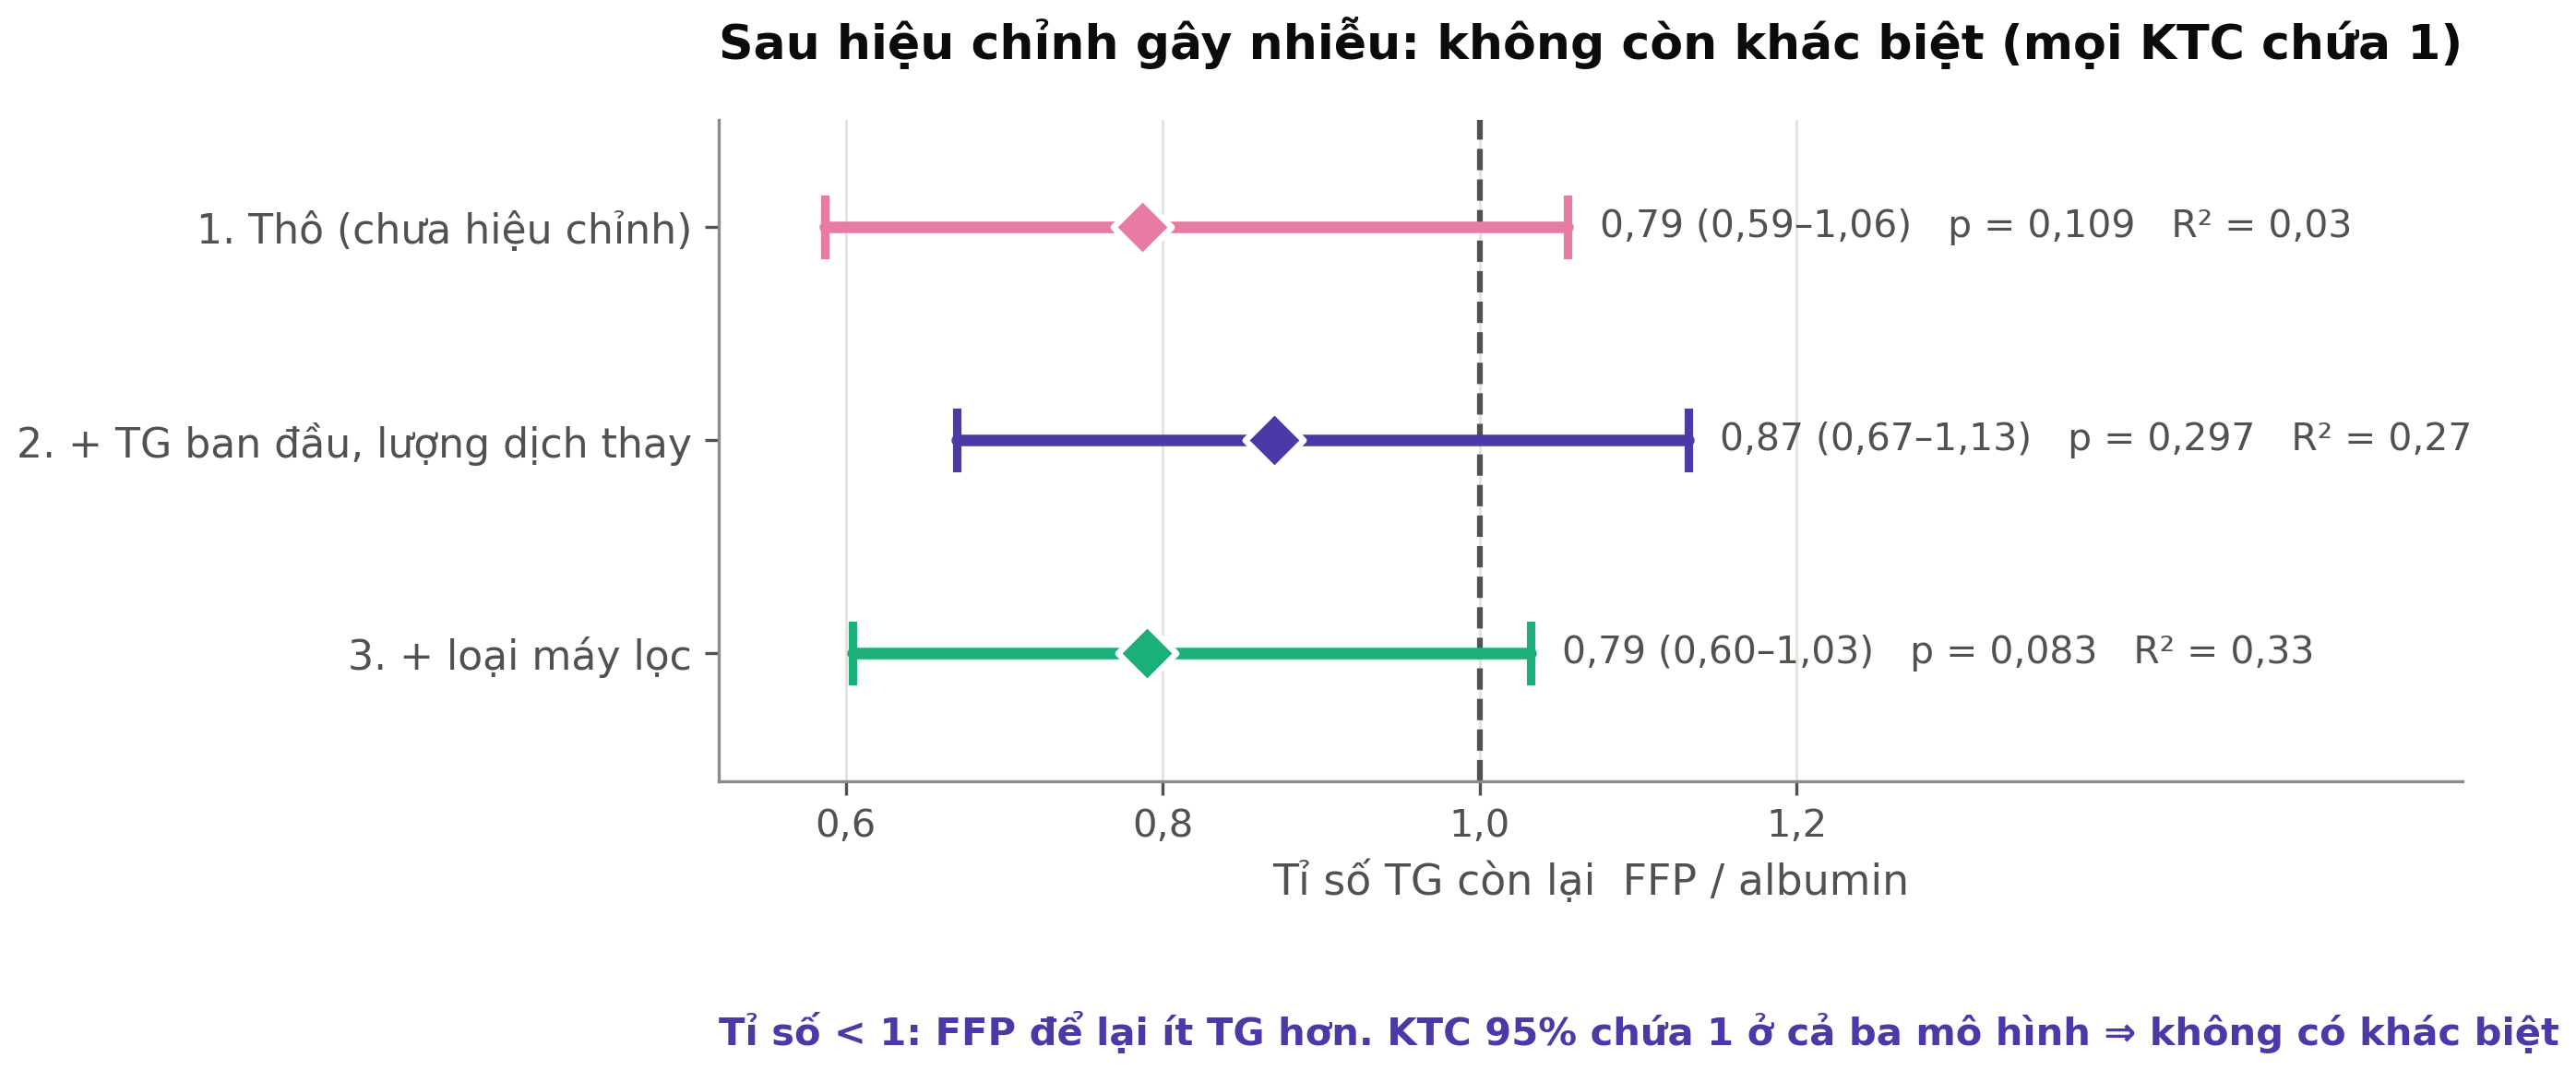
\includegraphics[width=\linewidth]{f8_adjusted.png}
		\figcap{\textbf{Hình 5.} Hồi quy log-tuyến tính. Hiệu chỉnh TG ban đầu và lượng dịch thay
		đưa tỉ số FFP/albumin từ 0,79 về \textbf{0,87} và $R^{2}$ từ 0,03 lên 0,27.}
		\end{minipage}%
		\hfill
		\begin{minipage}[t]{0.382\linewidth}\vspace{0pt}
		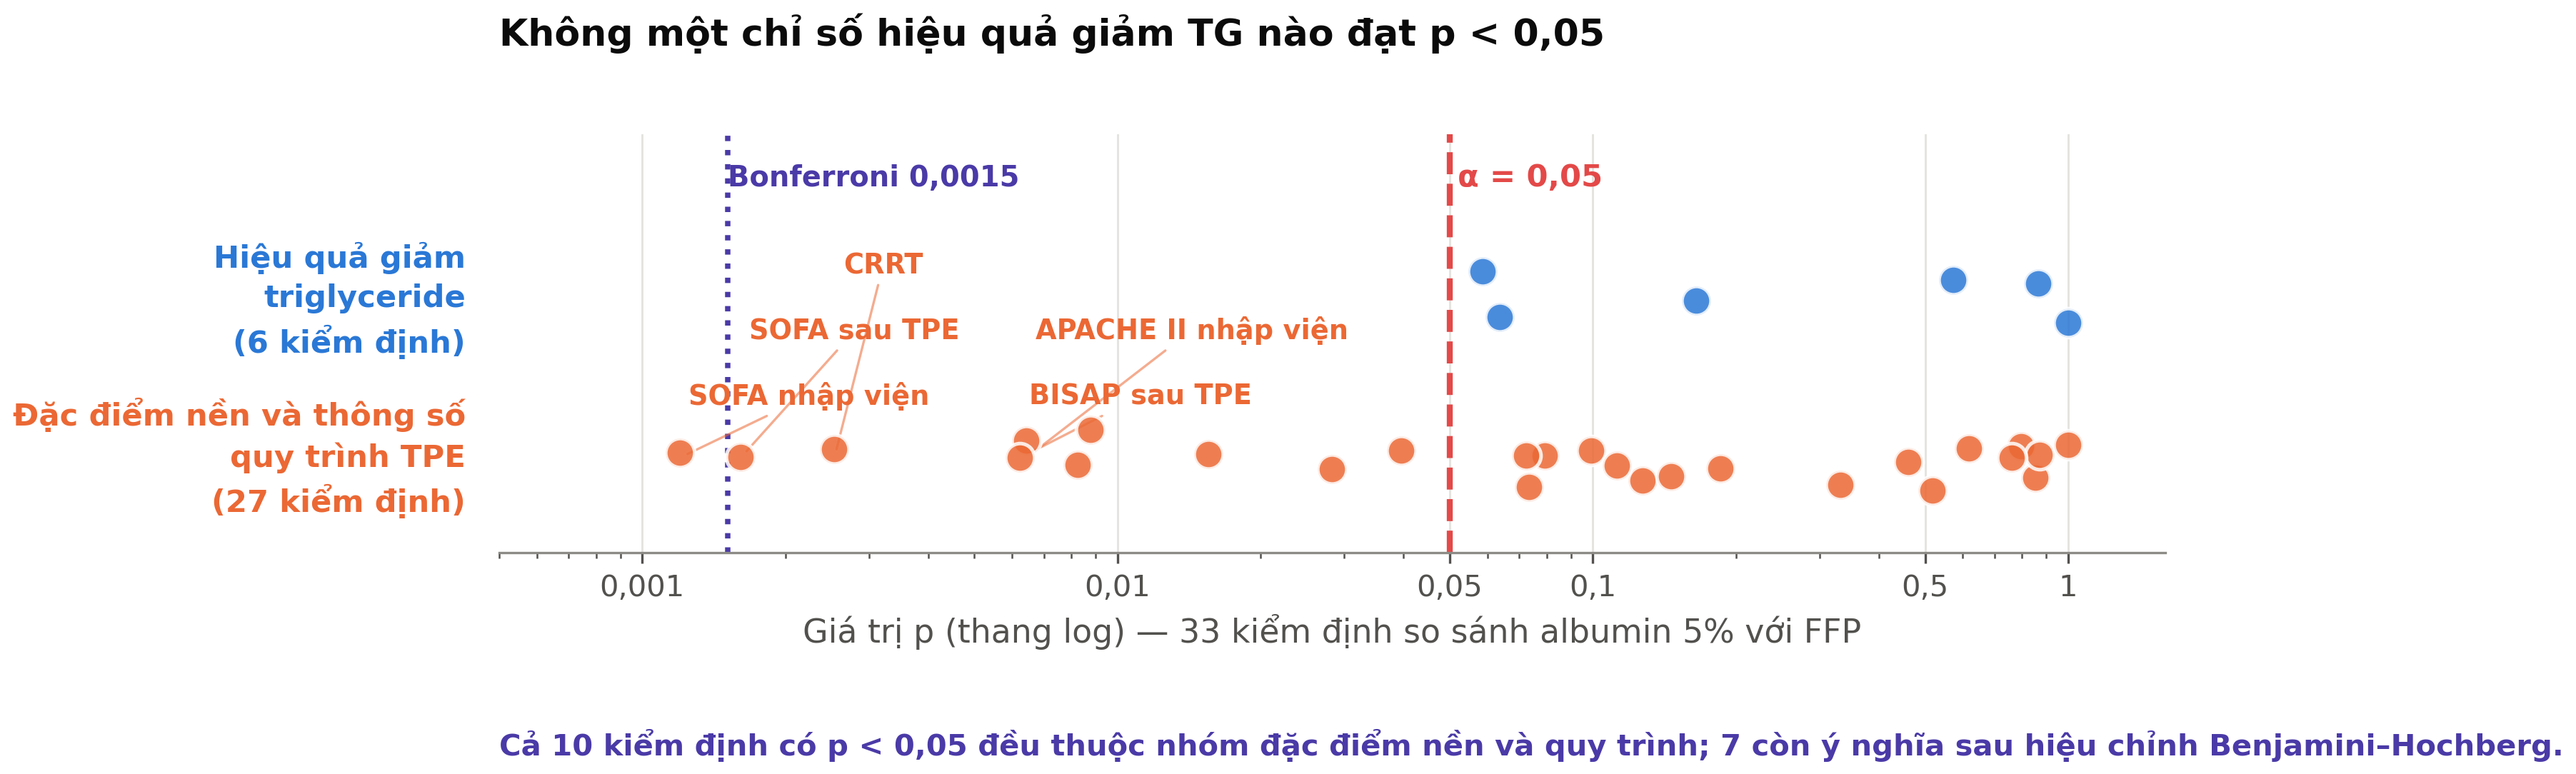
\includegraphics[width=\linewidth]{f9_pvalue_strip.png}
		\figcap{\textbf{Hình 6.} 33 kiểm định so sánh hai nhóm, xếp theo nhóm biến. \textbf{Không}
		chỉ số hiệu quả giảm TG nào đạt $p<0{,}05$.}
		\end{minipage}%
		\hfill
		\begin{minipage}[t]{0.255\linewidth}\vspace{0pt}
		\colorbox{lmagenta}{\begin{minipage}{0.92\linewidth}\raggedright\vspace{0.3em}
		\bignum{Tỉ số TG còn lại, thô}{0,79}{cgrey}
		\bignum{Sau hiệu chỉnh}{0,87}{cmagenta}
		\bignum{KTC 95\%}{0,67 -- 1,13}{cgrey}
		\bignum{Chênh tỉ lệ giảm}{$+4,1$ điểm \%}{cmagenta}
		{\scriptsize\textcolor{cgrey}{KTC 95\% $-0{,}9$ đến $9{,}2$; $p=0{,}059$}}
		\vspace{0.3em}\end{minipage}}
		\end{minipage}

		\vspace{0.15em}
		{\small \textcolor{cmagenta}{$\blacktriangleright$} \ \textbf{Chuỗi suy luận:}
		nhóm FFP \emph{nặng hơn ngay từ đầu} (SOFA 5,6 so với 3,4 \ $\cdot$ \ APACHE II 20,1 so với
		15,1 \ $\cdot$ \ CRRT 79\% so với 48\%; đều $p<0{,}01$) $\Rightarrow$ đây là \key{gây nhiễu do
		chỉ định}, không phải bằng chứng về hiệu quả lọc. Sau hiệu chỉnh, KTC của chênh lệch vẫn
		chứa 0: kết luận đúng là \textbf{"chưa thấy khác biệt"}, không phải "không có khác biệt".}
	}

	%=========================================================================
	% HÀNG 5 — KẾT LUẬN  |  ĐỘ VỮNG
	%=========================================================================
	\headerbox{\ \ Kết luận và đóng góp}{name=conclusion,column=0,span=2,row=0,below=kq3,
		headerColorOne=cgreen,borderColor=cgreen}{
		{\small
		\begin{enumerate}\compresslist
			\item[\textcolor{cgreen}{\textbf{1.}}] \textbf{Chọn phép kiểm theo dữ liệu.}
			      12/18 biến định lượng lệch chuẩn, và khác biệt không chỉ mang tính hình thức:
			      với số ngày nằm viện, $t$-test cho $p=0{,}014$ còn Wilcoxon cho $p=0{,}146$ ---
			      hai kết luận trái ngược trên cùng một bộ số.
			\item[\textcolor{cgreen}{\textbf{2.}}] \textbf{Dự báo rủi ro.} Chỉ BISAP $\geq3$
			      còn ý nghĩa sau hiệu chỉnh (OR 5,68; KTC 1,33--24,27); mô hình giải thích 19\%
			      biến thiên. Với 2,5 biến cố trên mỗi biến số, đây là kết quả thăm dò.
			\item[\textcolor{cgreen}{\textbf{3.}}] \textbf{Hiệu quả TPE được khẳng định chắc chắn}
			      bằng phân tích bắt cặp: TG giảm 77,8\% và cả ba thang điểm nặng đều cải thiện
			      ($p<0{,}001$), nhất quán ở hai loại dịch.
			\item[\textcolor{cgreen}{\textbf{4.}}] \textbf{Khác biệt thô giữa hai dịch là ảo ảnh
			      của yếu tố gây nhiễu} --- ba lớp kiểm chứng độc lập (hiệu chỉnh hồi quy, kiểm soát
			      đa so sánh, 11 kịch bản độ vững) đều dẫn tới cùng kết luận.
			\item[\textcolor{cgreen}{\textbf{5.}}] \textbf{Đóng góp phương pháp:} một khung phân
			      tích \hl{tái lập được} cho nghiên cứu quan sát cỡ nhỏ trong hồi sức.
			      \textbf{Hạn chế:} hồi cứu, không ngẫu nhiên; biến phân độ nặng tính từ nhịp tim,
			      nhịp thở và urê nên \textbf{không phải} Atlanta 2012; TPE lần 2 chỉ 13 ca.
			      \textbf{Hướng tiếp theo:} ghép cặp theo điểm xu hướng, mô hình hiệu ứng hỗn hợp.
		\end{enumerate}
}
	}

	\headerbox{\ \ Phân tích độ vững}{name=robust,column=2,row=0,below=kq3,
		headerColorOne=cgrey,borderColor=cgrey}{
		\centering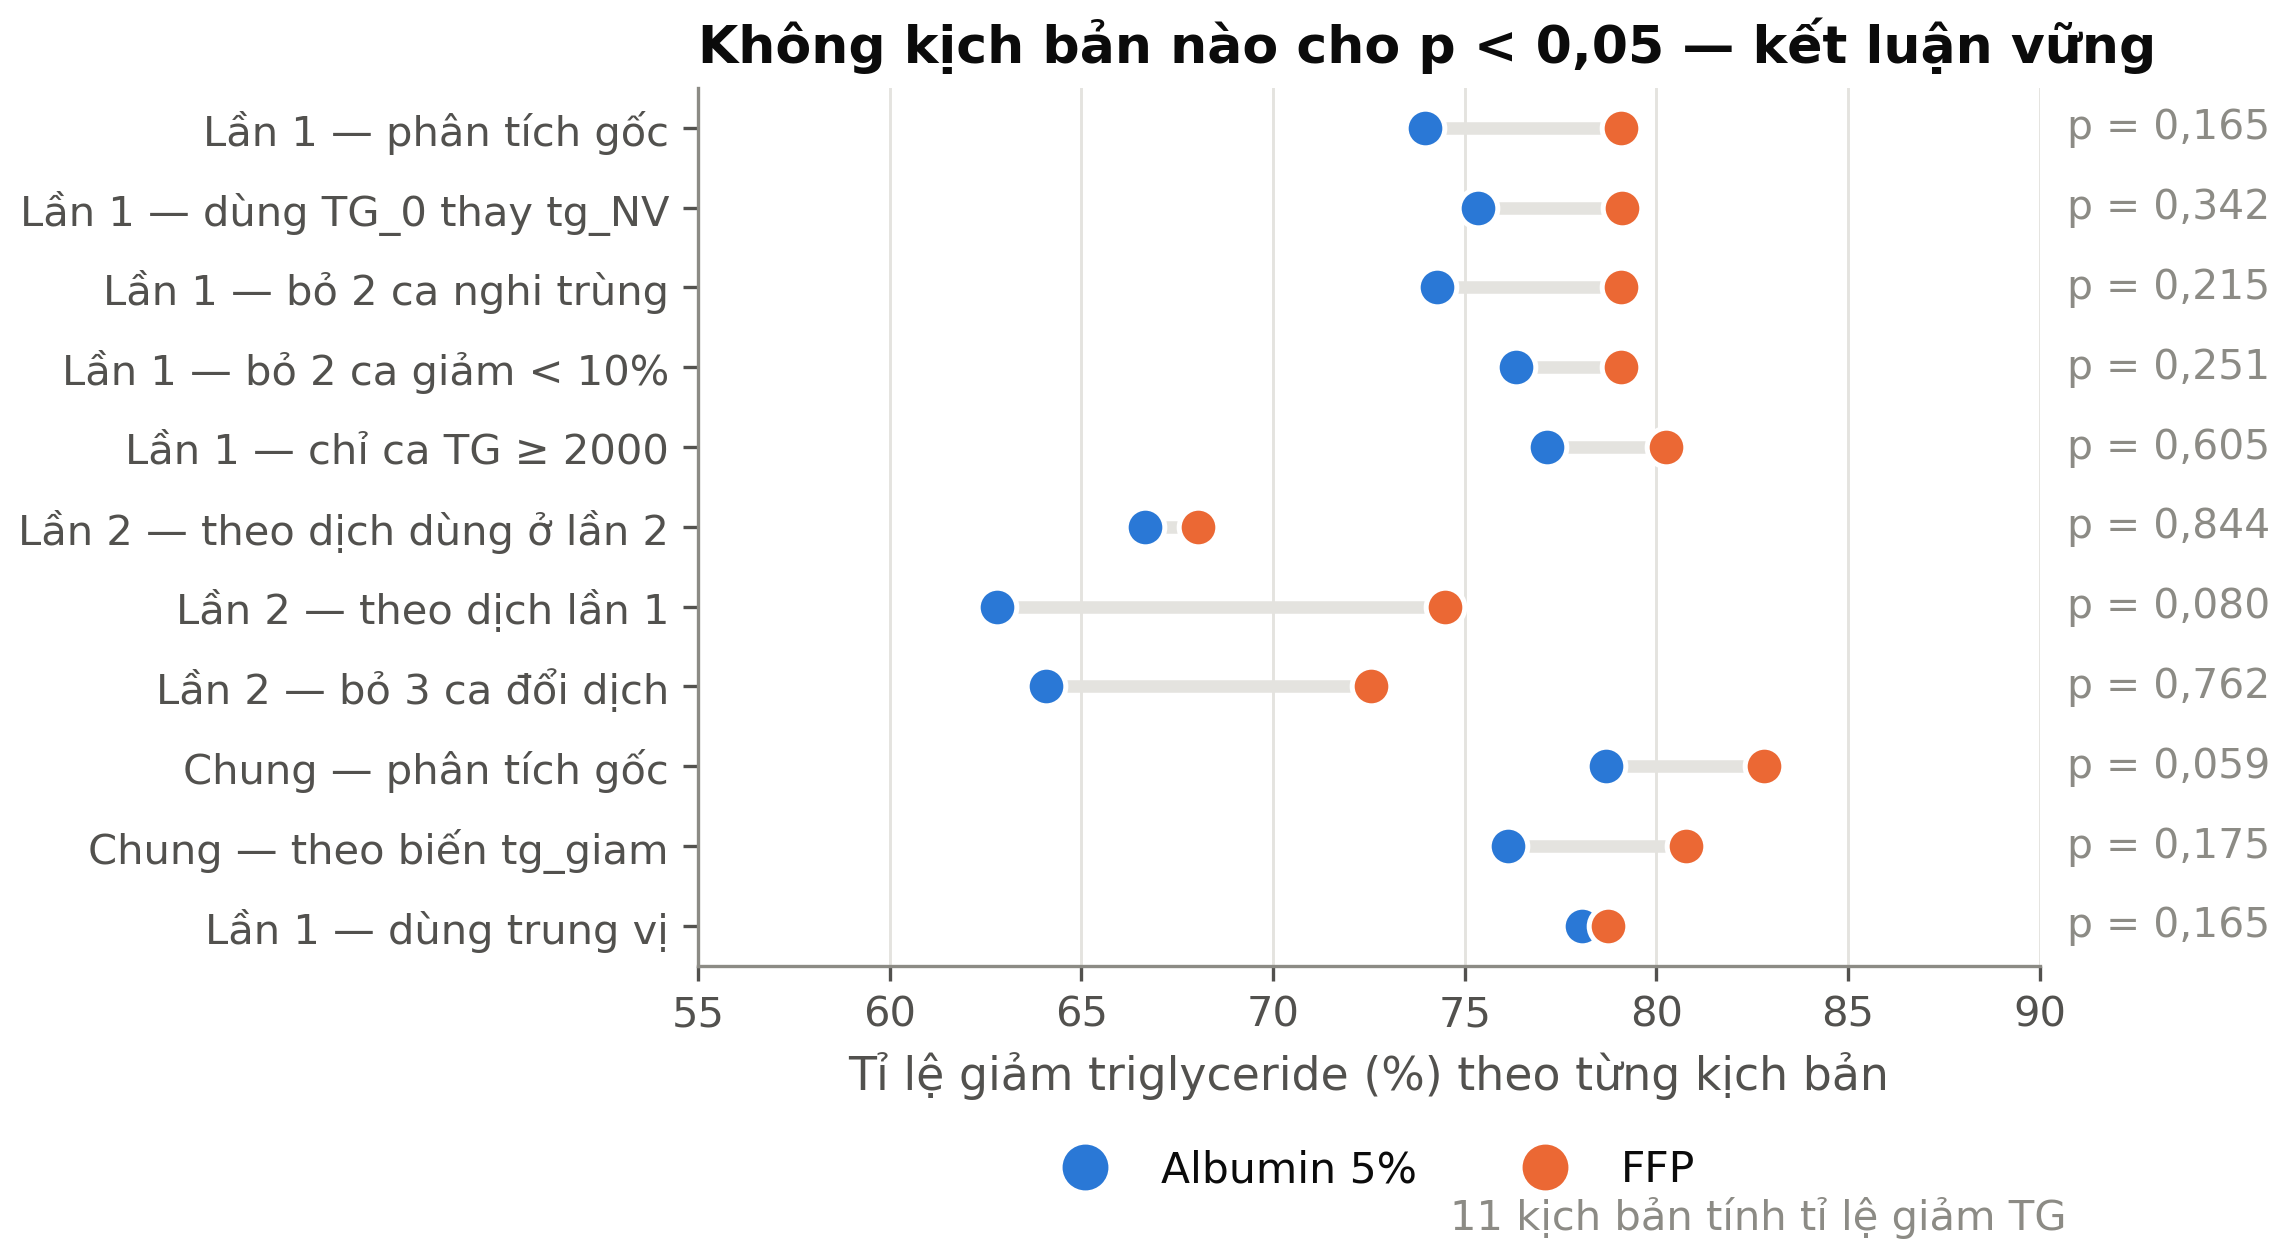
\includegraphics[width=0.89\linewidth]{f10_sensitivity.png}
		\par\raggedright
		\figcap{\textbf{Hình 7.} Tỉ lệ giảm TG tính lại theo 11 cách.
		\textbf{Không kịch bản nào} cho $p<0{,}05$.}
	}

	%=========================================================================
	% HÀNG 6 — TÀI LIỆU THAM KHẢO
	%=========================================================================
	\headerbox{\ \ Tài liệu tham khảo}{name=ref,column=0,span=3,row=0,below=robust,
		headerColorOne=cgrey,borderColor=cgrey}{
		\scriptsize
		\begin{multicols}{3}
		\renewcommand{\refname}{\vspace{-1ex}}
		\begin{thebibliography}{9}\compresslist
			\bibitem{lilliefors} Lilliefors H.W.
			\emph{On the Kolmogorov--Smirnov test for normality with mean and variance unknown.}
			J Am Stat Assoc, 62(318):399--402, 1967.
			\bibitem{nagelkerke} Nagelkerke N.J.D.
			\emph{A note on a general definition of the coefficient of determination.}
			Biometrika, 78(3):691--692, 1991.
			\bibitem{bh} Benjamini Y., Hochberg Y.
			\emph{Controlling the false discovery rate: a practical and powerful approach to
			multiple testing.} J R Stat Soc Series B, 57(1):289--300, 1995.
			\bibitem{peduzzi} Peduzzi P., Concato J., Kemper E., Holford T.R., Feinstein A.R.
			\emph{A simulation study of the number of events per variable in logistic regression
			analysis.} J Clin Epidemiol, 49(12):1373--1379, 1996.
			\bibitem{atlanta} Banks P.A. và cs.
			\emph{Classification of acute pancreatitis --- 2012: revision of the Atlanta
			classification and definitions by international consensus.} Gut, 62(1):102--111, 2013.
			\bibitem{asfa} Padmanabhan A. và cs.
			\emph{Guidelines on the use of therapeutic apheresis in clinical practice.}
			J Clin Apher, 34(3):171--354, 2019.
		\end{thebibliography}
		\end{multicols}
	}

	\end{poster}

\end{document}
